
\subsection{Velocity field}

The velocity field for the Smith-Hutton case, given by $\vb{v} = 2 y (1 - x^2) \vb{i} - 2 x (1 - y^2) \vb{j}$ and verifies the incompressibility condition since $\div{\vb{v}} = 0$. 

The only points where $\vb{v}$ vanishes are $(0,0)$, $(-1,1)$, $(1,1)$, $(-1,-1)$ and $(1,-1)$. If $L < 1$, then only $(0,0)$ belongs to $\overline{\Omega}$. If $L > 1$, the first three points belong to $\overline{\Omega}$. 

In this and in the coming sections we will assume $L = 1$. The stream function associated to $\vb{v}$ is $\psi(x,y) = -(1-x^2)(1-y^2)$. Recall that the streamlines are defined to be the curves $C \subset \Omega$ tangent to the vector field $\vb{v}$ at each point. Let $h \colon I \subset \real \to \Omega$, $t \mapsto h(t) = (x(t), y(t))$ be the parametrization of a streamline. Then it satisfies the following system of ODEs:
\begin{equation} \label{eq:velocity_smith_hutton_odes}
	\left\{
	\begin{aligned}
		\dot{x}(t) &= 2 y (1 - x^2) \\
		\dot{y}(t) &= - 2 x (1 - y^2)
	\end{aligned}
	\right.
\end{equation}
Since at each point in $\Omega$ there is a unique velocity vector, each point is contained in a single streamline. In order to find the streamlines, we can specify an initial condition $(x_0, y_0) \in \Omega$ and then pose an initial value problem with the system \eqref{eq:velocity_smith_hutton_odes}. The streamlines must fill $\Omega$ since $\vb{v}$ is defined everywhere, hence $(x_0, y_0) \in \Omega$ is arbitrary. However, we may become less formal and take $x_0 \in (-L, 0)$ and $y_0 = 0$. With this in mind, the resulting initial value problem for the streamlines is the following:
\begin{equation} \label{eq:velocity_smith_hutton_ivp}
	\left\{
	\begin{aligned}
		\dot{x}(t) &= 2 y (1 - x^2) 	&	x(0) &= x_0 \\
		\dot{y}(t) &= - 2 x (1 - y^2)	&	y(0) &= 0
	\end{aligned}
	\right.
\end{equation}
Finding a solution to \eqref{eq:velocity_smith_hutton_ivp} might be difficult as the system is non--linear. Nonetheless, even more important than finding an explicit formula that solves the initial value problem is proving the existence and uniqueness of solution. To do so, we define the following vector field:
\begin{equation}
	\begin{aligned}
		f \colon \Omega \subset \real^2 &\longrightarrow \real^2 \\
		(x,y) &\longmapsto f(x,y) = 
		\begin{pmatrix}
			2 y (1 - x^2) \\ - 2 x (1 - y^2)
		\end{pmatrix}
	\end{aligned}
\end{equation}
Then the problem \eqref{eq:velocity_smith_hutton_ivp} is rewritten as:
\begin{equation} \label{eq:velocity_smith_hutton_ivp_2}
	\frac{\dd}{\dd{t}} 
	\begin{pmatrix}
		x(t) \\ y(t)
	\end{pmatrix} = 
	f(x,y)	
	\quad
	\begin{pmatrix}
		x(0) \\ y(0)
	\end{pmatrix} =
	\begin{pmatrix}
		x_0 \\ 0
	\end{pmatrix}
\end{equation}
The ODE \eqref{eq:velocity_smith_hutton_ivp_2} is autonomous since $f$ does not depend upon time. Let $U \subset \real^2$ be an open bounded convex subset containing $\Omega \cup \left([-L, L] \times \{ 0 \} \right)$ (for instance, the ball $B(\vb{0}, 3)$). The vector field $f$ is actually defined on all $\real^2$ and is a $\mathcal{C}^\infty(\real^2, \real^2)$ map and, in particular, is a $\mathcal{C}^1(\overline{U}, \real^2)$ map. By theorem \ref{teo:c1_function_implies_lipschitz}, $f$ is Lipschitz on $\overline{U}$. By the Picard--Lindelöf theorem (Theorem \ref{teo:picard_lindelof}), the solution of \eqref{eq:velocity_smith_hutton_ivp} exists and is unique.

Once we have proven that a solution to \eqref{eq:velocity_smith_hutton_ivp} exists and is unique, we aim to find the solution for several $x_0 \in (-L, 0)$. As we have previously mentioned, we cannot expect to find an analytical solution since the ODE is non--linear. Nevertheless we may apply a numerical method, such as the Runge--Kutta 4 algorithm to sort out the problem. This is precisely what has been done to produce figure \ref{fig:smith_hutton_N201_streamlines}. In it, the norm of the vector field $\vb{v}$ is shown, along with the streamlines for several $x_0$ values.

\begin{figure}[ht]
	\centering
	%	\fbox{% GNUPLOT: LaTeX picture with Postscript
\begingroup
  % Encoding inside the plot.  In the header of your document, this encoding
  % should to defined, e.g., by using
  % \usepackage[cp1252,<other encodings>]{inputenc}
  \inputencoding{cp1252}%
  \makeatletter
  \providecommand\color[2][]{%
    \GenericError{(gnuplot) \space\space\space\@spaces}{%
      Package color not loaded in conjunction with
      terminal option `colourtext'%
    }{See the gnuplot documentation for explanation.%
    }{Either use 'blacktext' in gnuplot or load the package
      color.sty in LaTeX.}%
    \renewcommand\color[2][]{}%
  }%
  \providecommand\includegraphics[2][]{%
    \GenericError{(gnuplot) \space\space\space\@spaces}{%
      Package graphicx or graphics not loaded%
    }{See the gnuplot documentation for explanation.%
    }{The gnuplot epslatex terminal needs graphicx.sty or graphics.sty.}%
    \renewcommand\includegraphics[2][]{}%
  }%
  \providecommand\rotatebox[2]{#2}%
  \@ifundefined{ifGPcolor}{%
    \newif\ifGPcolor
    \GPcolortrue
  }{}%
  \@ifundefined{ifGPblacktext}{%
    \newif\ifGPblacktext
    \GPblacktextfalse
  }{}%
  % define a \g@addto@macro without @ in the name:
  \let\gplgaddtomacro\g@addto@macro
  % define empty templates for all commands taking text:
  \gdef\gplbacktext{}%
  \gdef\gplfronttext{}%
  \makeatother
  \ifGPblacktext
    % no textcolor at all
    \def\colorrgb#1{}%
    \def\colorgray#1{}%
  \else
    % gray or color?
    \ifGPcolor
      \def\colorrgb#1{\color[rgb]{#1}}%
      \def\colorgray#1{\color[gray]{#1}}%
      \expandafter\def\csname LTw\endcsname{\color{white}}%
      \expandafter\def\csname LTb\endcsname{\color{black}}%
      \expandafter\def\csname LTa\endcsname{\color{black}}%
      \expandafter\def\csname LT0\endcsname{\color[rgb]{1,0,0}}%
      \expandafter\def\csname LT1\endcsname{\color[rgb]{0,1,0}}%
      \expandafter\def\csname LT2\endcsname{\color[rgb]{0,0,1}}%
      \expandafter\def\csname LT3\endcsname{\color[rgb]{1,0,1}}%
      \expandafter\def\csname LT4\endcsname{\color[rgb]{0,1,1}}%
      \expandafter\def\csname LT5\endcsname{\color[rgb]{1,1,0}}%
      \expandafter\def\csname LT6\endcsname{\color[rgb]{0,0,0}}%
      \expandafter\def\csname LT7\endcsname{\color[rgb]{1,0.3,0}}%
      \expandafter\def\csname LT8\endcsname{\color[rgb]{0.5,0.5,0.5}}%
    \else
      % gray
      \def\colorrgb#1{\color{black}}%
      \def\colorgray#1{\color[gray]{#1}}%
      \expandafter\def\csname LTw\endcsname{\color{white}}%
      \expandafter\def\csname LTb\endcsname{\color{black}}%
      \expandafter\def\csname LTa\endcsname{\color{black}}%
      \expandafter\def\csname LT0\endcsname{\color{black}}%
      \expandafter\def\csname LT1\endcsname{\color{black}}%
      \expandafter\def\csname LT2\endcsname{\color{black}}%
      \expandafter\def\csname LT3\endcsname{\color{black}}%
      \expandafter\def\csname LT4\endcsname{\color{black}}%
      \expandafter\def\csname LT5\endcsname{\color{black}}%
      \expandafter\def\csname LT6\endcsname{\color{black}}%
      \expandafter\def\csname LT7\endcsname{\color{black}}%
      \expandafter\def\csname LT8\endcsname{\color{black}}%
    \fi
  \fi
    \setlength{\unitlength}{0.0500bp}%
    \ifx\gptboxheight\undefined%
      \newlength{\gptboxheight}%
      \newlength{\gptboxwidth}%
      \newsavebox{\gptboxtext}%
    \fi%
    \setlength{\fboxrule}{0.5pt}%
    \setlength{\fboxsep}{1pt}%
    \definecolor{tbcol}{rgb}{1,1,1}%
\begin{picture}(7370.00,3968.00)%
    \gplgaddtomacro\gplbacktext{%
      \csname LTb\endcsname%%
      \put(814,719){\makebox(0,0)[r]{\strut{}0.0}}%
      \put(814,1234){\makebox(0,0)[r]{\strut{}0.2}}%
      \put(814,1748){\makebox(0,0)[r]{\strut{}0.4}}%
      \put(814,2263){\makebox(0,0)[r]{\strut{}0.6}}%
      \put(814,2777){\makebox(0,0)[r]{\strut{}0.8}}%
      \put(814,3292){\makebox(0,0)[r]{\strut{}1.0}}%
      \put(946,499){\makebox(0,0){\strut{}-1.0}}%
      \put(2233,499){\makebox(0,0){\strut{}-0.5}}%
      \put(3520,499){\makebox(0,0){\strut{}0.0}}%
      \put(4806,499){\makebox(0,0){\strut{}0.5}}%
      \put(6093,499){\makebox(0,0){\strut{}1.0}}%
    }%
    \gplgaddtomacro\gplfronttext{%
      \csname LTb\endcsname%%
      \put(209,2005){\rotatebox{-270}{\makebox(0,0){\strut{}$y \ (\mathrm{m})$}}}%
      \put(3519,169){\makebox(0,0){\strut{}$x \ (\mathrm{m})$}}%
      \csname LTb\endcsname%%
      \put(6611,719){\makebox(0,0)[l]{\strut{}0.0}}%
      \put(6611,1362){\makebox(0,0)[l]{\strut{}0.5}}%
      \put(6611,2005){\makebox(0,0)[l]{\strut{}1.0}}%
      \put(6611,2648){\makebox(0,0)[l]{\strut{}1.5}}%
      \put(6611,3292){\makebox(0,0)[l]{\strut{}2.0}}%
      \put(7073,2005){\rotatebox{-270}{\makebox(0,0){\strut{}$\phi$}}}%
      \put(3519,3622){\makebox(0,0){\strut{}\textbf{Smith--Hutton case} $(\mathrm{Pe} = 10^{2})$}}%
    }%
    \gplbacktext
    \put(0,0){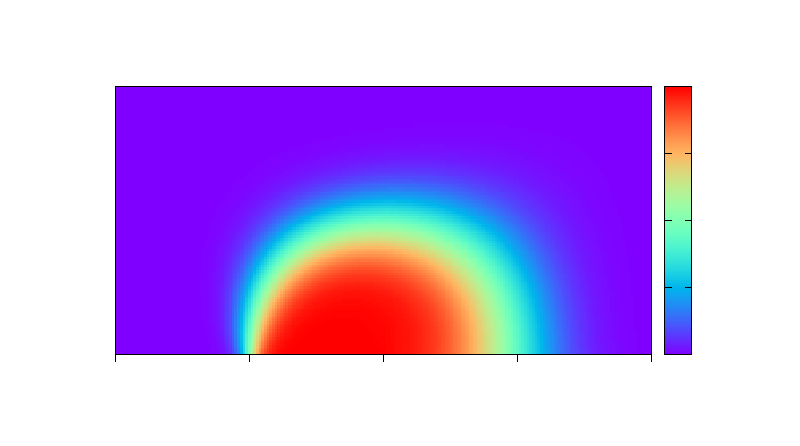
\includegraphics[width={368.50bp},height={198.40bp}]{figures/case_smith_hutton/smith_hutton_N201_Pe1.0e+02}}%
    \gplfronttext
  \end{picture}%
\endgroup
}
	% GNUPLOT: LaTeX picture with Postscript
\begingroup
  % Encoding inside the plot.  In the header of your document, this encoding
  % should to defined, e.g., by using
  % \usepackage[cp1252,<other encodings>]{inputenc}
  \inputencoding{cp1252}%
  \makeatletter
  \providecommand\color[2][]{%
    \GenericError{(gnuplot) \space\space\space\@spaces}{%
      Package color not loaded in conjunction with
      terminal option `colourtext'%
    }{See the gnuplot documentation for explanation.%
    }{Either use 'blacktext' in gnuplot or load the package
      color.sty in LaTeX.}%
    \renewcommand\color[2][]{}%
  }%
  \providecommand\includegraphics[2][]{%
    \GenericError{(gnuplot) \space\space\space\@spaces}{%
      Package graphicx or graphics not loaded%
    }{See the gnuplot documentation for explanation.%
    }{The gnuplot epslatex terminal needs graphicx.sty or graphics.sty.}%
    \renewcommand\includegraphics[2][]{}%
  }%
  \providecommand\rotatebox[2]{#2}%
  \@ifundefined{ifGPcolor}{%
    \newif\ifGPcolor
    \GPcolortrue
  }{}%
  \@ifundefined{ifGPblacktext}{%
    \newif\ifGPblacktext
    \GPblacktextfalse
  }{}%
  % define a \g@addto@macro without @ in the name:
  \let\gplgaddtomacro\g@addto@macro
  % define empty templates for all commands taking text:
  \gdef\gplbacktext{}%
  \gdef\gplfronttext{}%
  \makeatother
  \ifGPblacktext
    % no textcolor at all
    \def\colorrgb#1{}%
    \def\colorgray#1{}%
  \else
    % gray or color?
    \ifGPcolor
      \def\colorrgb#1{\color[rgb]{#1}}%
      \def\colorgray#1{\color[gray]{#1}}%
      \expandafter\def\csname LTw\endcsname{\color{white}}%
      \expandafter\def\csname LTb\endcsname{\color{black}}%
      \expandafter\def\csname LTa\endcsname{\color{black}}%
      \expandafter\def\csname LT0\endcsname{\color[rgb]{1,0,0}}%
      \expandafter\def\csname LT1\endcsname{\color[rgb]{0,1,0}}%
      \expandafter\def\csname LT2\endcsname{\color[rgb]{0,0,1}}%
      \expandafter\def\csname LT3\endcsname{\color[rgb]{1,0,1}}%
      \expandafter\def\csname LT4\endcsname{\color[rgb]{0,1,1}}%
      \expandafter\def\csname LT5\endcsname{\color[rgb]{1,1,0}}%
      \expandafter\def\csname LT6\endcsname{\color[rgb]{0,0,0}}%
      \expandafter\def\csname LT7\endcsname{\color[rgb]{1,0.3,0}}%
      \expandafter\def\csname LT8\endcsname{\color[rgb]{0.5,0.5,0.5}}%
    \else
      % gray
      \def\colorrgb#1{\color{black}}%
      \def\colorgray#1{\color[gray]{#1}}%
      \expandafter\def\csname LTw\endcsname{\color{white}}%
      \expandafter\def\csname LTb\endcsname{\color{black}}%
      \expandafter\def\csname LTa\endcsname{\color{black}}%
      \expandafter\def\csname LT0\endcsname{\color{black}}%
      \expandafter\def\csname LT1\endcsname{\color{black}}%
      \expandafter\def\csname LT2\endcsname{\color{black}}%
      \expandafter\def\csname LT3\endcsname{\color{black}}%
      \expandafter\def\csname LT4\endcsname{\color{black}}%
      \expandafter\def\csname LT5\endcsname{\color{black}}%
      \expandafter\def\csname LT6\endcsname{\color{black}}%
      \expandafter\def\csname LT7\endcsname{\color{black}}%
      \expandafter\def\csname LT8\endcsname{\color{black}}%
    \fi
  \fi
    \setlength{\unitlength}{0.0500bp}%
    \ifx\gptboxheight\undefined%
      \newlength{\gptboxheight}%
      \newlength{\gptboxwidth}%
      \newsavebox{\gptboxtext}%
    \fi%
    \setlength{\fboxrule}{0.5pt}%
    \setlength{\fboxsep}{1pt}%
    \definecolor{tbcol}{rgb}{1,1,1}%
\begin{picture}(7370.00,3968.00)%
    \gplgaddtomacro\gplbacktext{%
      \csname LTb\endcsname%%
      \put(814,733){\makebox(0,0)[r]{\strut{}$0$}}%
      \put(814,1242){\makebox(0,0)[r]{\strut{}$0.2$}}%
      \put(814,1751){\makebox(0,0)[r]{\strut{}$0.4$}}%
      \put(814,2260){\makebox(0,0)[r]{\strut{}$0.6$}}%
      \put(814,2769){\makebox(0,0)[r]{\strut{}$0.8$}}%
      \put(814,3278){\makebox(0,0)[r]{\strut{}$1$}}%
      \put(1009,513){\makebox(0,0){\strut{}-1.0}}%
      \put(2282,513){\makebox(0,0){\strut{}-0.5}}%
      \put(3554,513){\makebox(0,0){\strut{}0.0}}%
      \put(4827,513){\makebox(0,0){\strut{}0.5}}%
      \put(6099,513){\makebox(0,0){\strut{}1.0}}%
    }%
    \gplgaddtomacro\gplfronttext{%
      \csname LTb\endcsname%%
      \put(209,2005){\rotatebox{-270}{\makebox(0,0){\strut{}$y \ (\mathrm{m})$}}}%
      \put(3554,183){\makebox(0,0){\strut{}$x \ (\mathrm{m})$}}%
      \csname LTb\endcsname%%
      \put(6612,733){\makebox(0,0)[l]{\strut{}0.0}}%
      \put(6612,1369){\makebox(0,0)[l]{\strut{}0.5}}%
      \put(6612,2005){\makebox(0,0)[l]{\strut{}1.0}}%
      \put(6612,2641){\makebox(0,0)[l]{\strut{}1.5}}%
      \put(6612,3278){\makebox(0,0)[l]{\strut{}2.0}}%
      \put(7074,2005){\rotatebox{-270}{\makebox(0,0){\strut{}$\norm{\vb{v}} \ (\mathrm{m} / \mathrm{s})$}}}%
      \put(3554,3608){\makebox(0,0){\strut{}\textbf{Smith--Hutton case -- Velocity field}}}%
    }%
    \gplbacktext
    \put(0,0){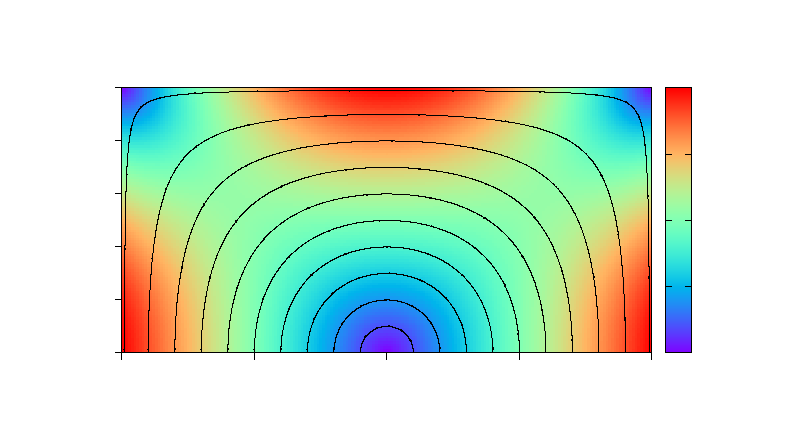
\includegraphics[width={368.50bp},height={198.40bp}]{figures/case_smith_hutton/smith_hutton_N201_streamlines}}%
    \gplfronttext
  \end{picture}%
\endgroup

	\captionsetup{width=0.75\textwidth}
	\caption{Norm of the Smith--Hutton velocity field and streamlines for $x_0 = 0.10, \ 0.20, \ 0.30, \ 0.40, \ 0.50, \ 0.60, \ 0.70, \ 0.80, \ 0.90$ and $0.99 \ \meter$. The vectors tangent to the streamlines are normalized and then scaled down by a factor of $\sqrt{2}/50$.}
	\label{fig:smith_hutton_N201_streamlines}
\end{figure}